%! Author = Mateusz Budzisz
%! Date = 26/05/2024

\chapter{Prezentacja systemu}
\label{ch:prezentacja-systemu}



\section{Widok głównej stron}
\label{sec:mapawidok}
\begin{figure}[H]
    \centering
    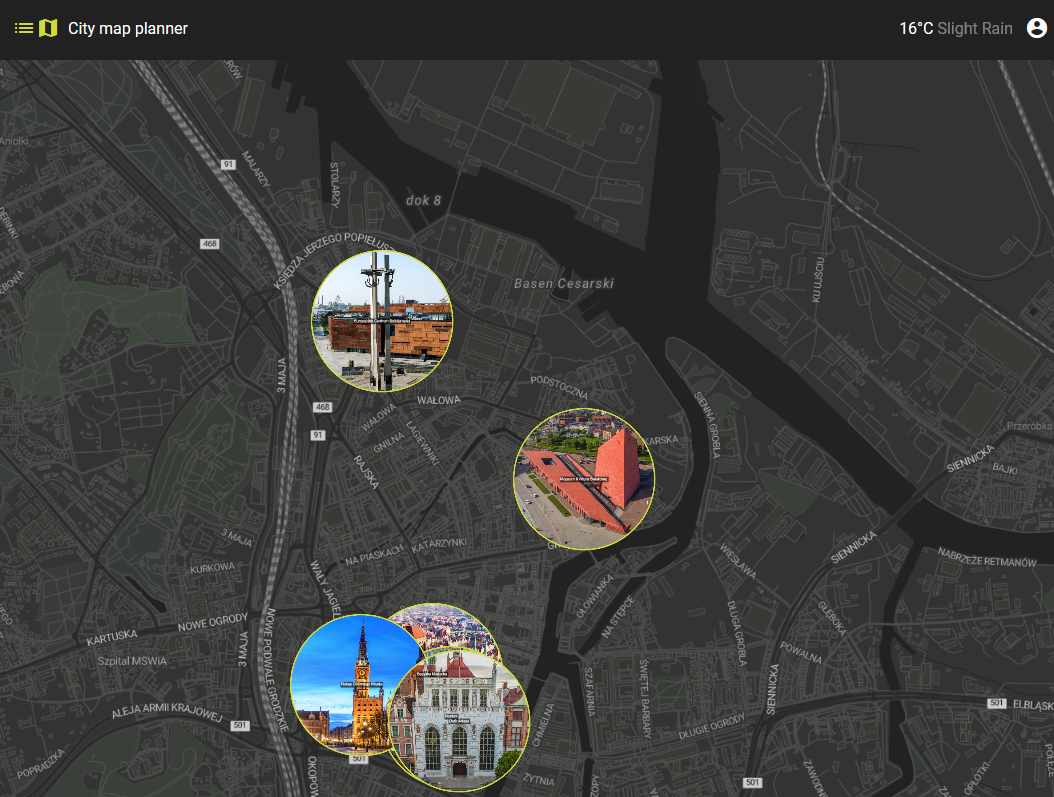
\includegraphics[width=1\textwidth]{attachments/mapawidok}
    \caption{Widok głównej strony}
    \label{fig:mapawidok}
    \end{figure}

\section{Widok pojedynczej atrakcji}
\label{sec:atrakcjawidok}
\begin{figure}[H]
        \centering
        \includegraphics[width=1\textwidth]{attachments/atrakcjawidok}
        \caption{Widok pojedynczej atrakcji}
        \label{fig:mapawidok}
\end{figure}

\section{Widok koszyka}
\label{sec:koszyk}
    \begin{figure}[H]
        \centering
        \includegraphics[width=1\textwidth]{attachments/koszyk}
        \caption{Widok koszyka}
        \label{fig:koszyk}
\end{figure}

\section{Widok kalendarza}
\label{sec:atrakcjawidok}
\begin{figure}[H]
        \centering
        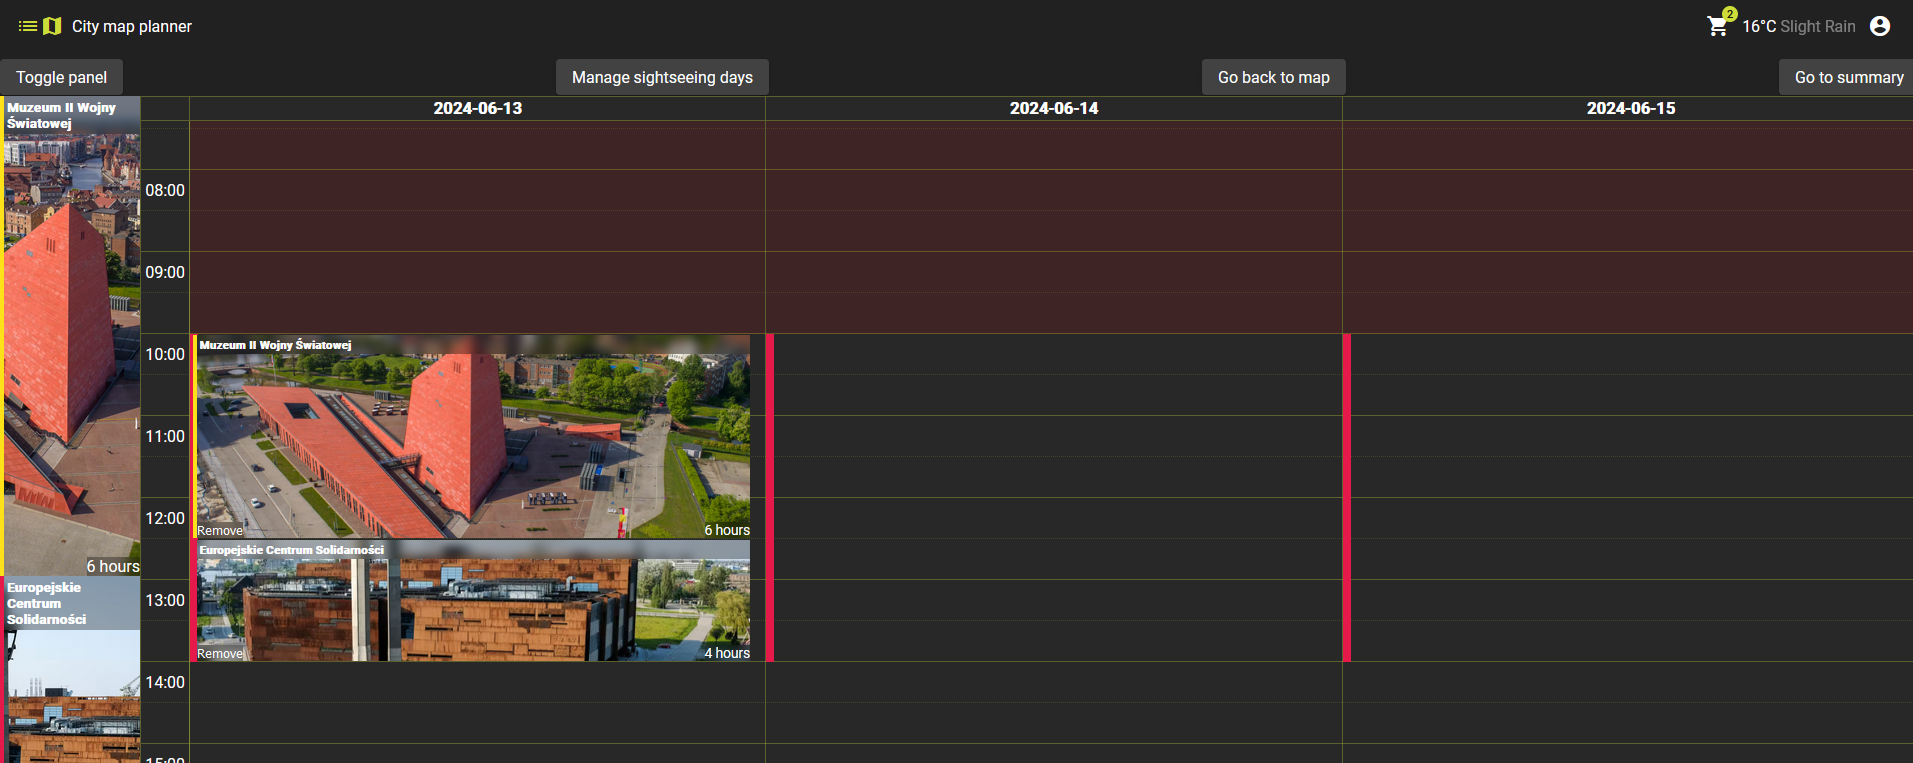
\includegraphics[width=1\textwidth]{attachments/kalendarz}
        \caption{Widok kalendarza}
        \label{fig:kalendarz}
\end{figure}
\section{Widok podsumowania}
\label{sec:atrakcjawidok}
\begin{figure}[H]
    \centering
    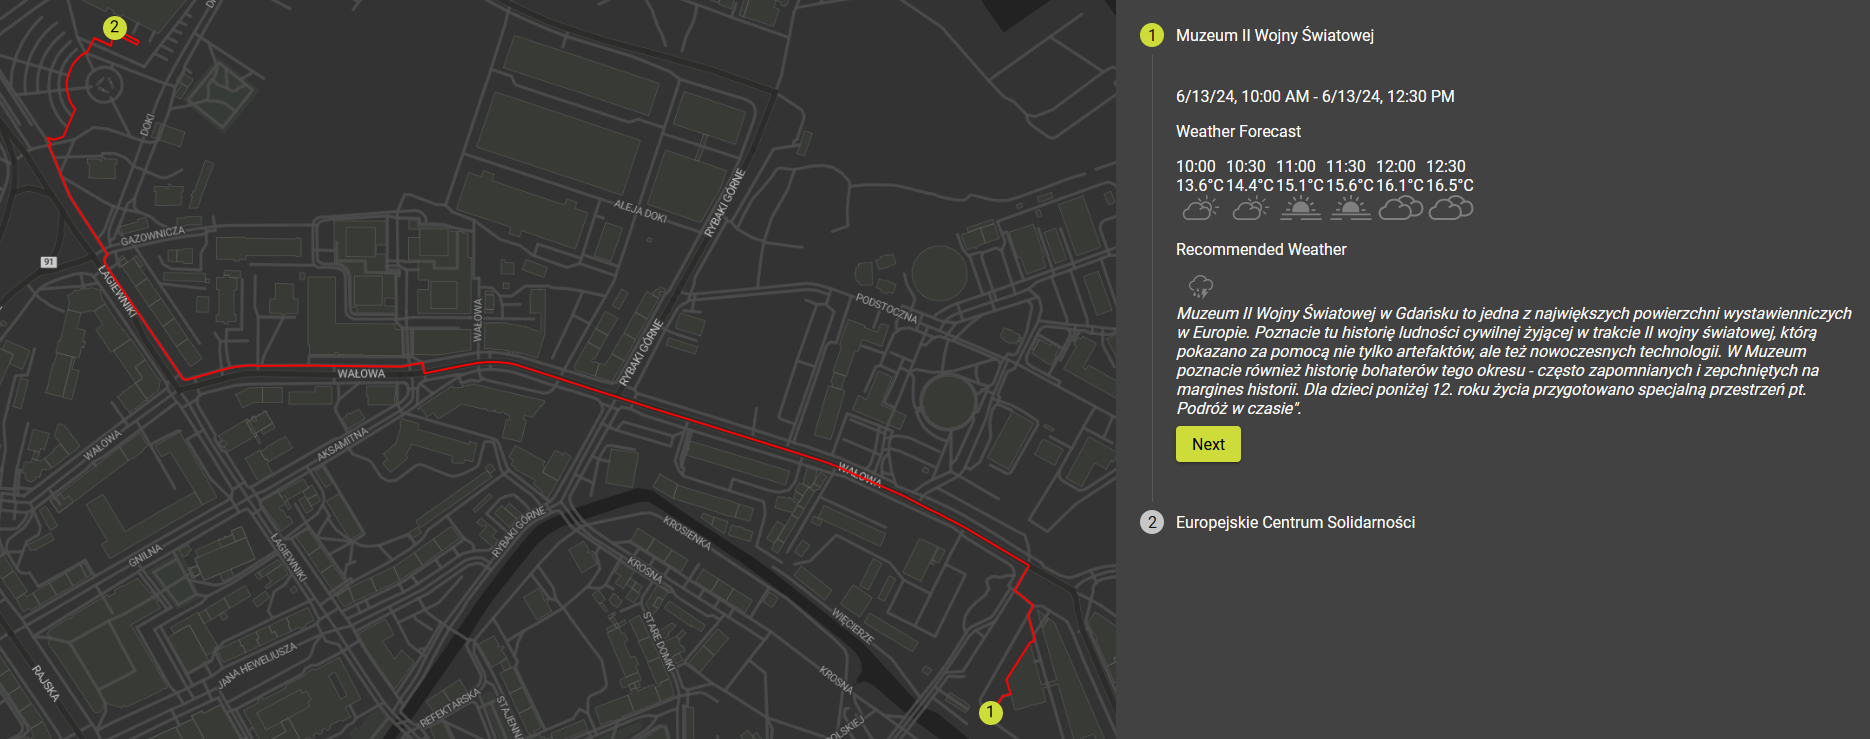
\includegraphics[width=1\textwidth]{attachments/podsumowanie}
    \caption{Widok podsumowanie}
    \label{fig:podsumowanie}
\end{figure}
\section{Widok Listy POI}
\label{sec:poilist}

\begin{figure}[H]
    \centering
    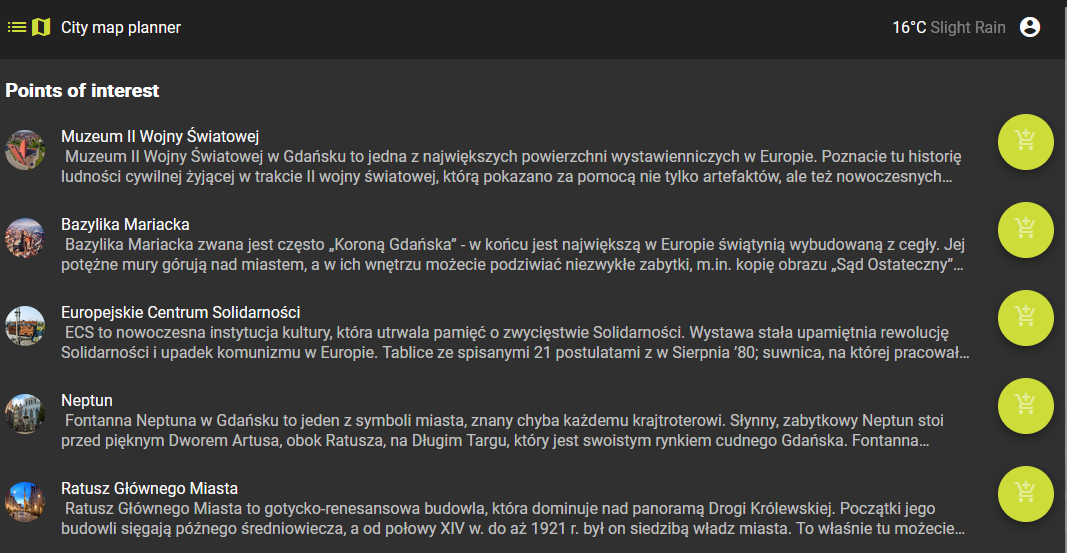
\includegraphics[width=1\textwidth]{attachments/poilist}
    \caption{Widok listy wszystkich dostępnych atrakcji}
    \label{fig:poilist}
\end{figure}


\section{Widok Listy POI}
\label{sec:user}

\begin{figure}[H]
    \centering
    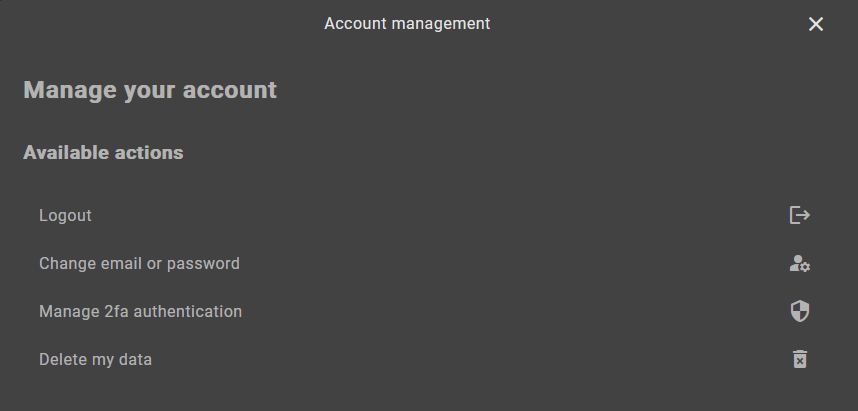
\includegraphics[width=1\textwidth]{attachments/user}
    \caption{Widok panelu zarządzania użytkownikiem}
    \label{fig:user}
\end{figure}

\section{Widok Logowania}
\label{sec:logowanie}

\begin{figure}[H]
    \centering
    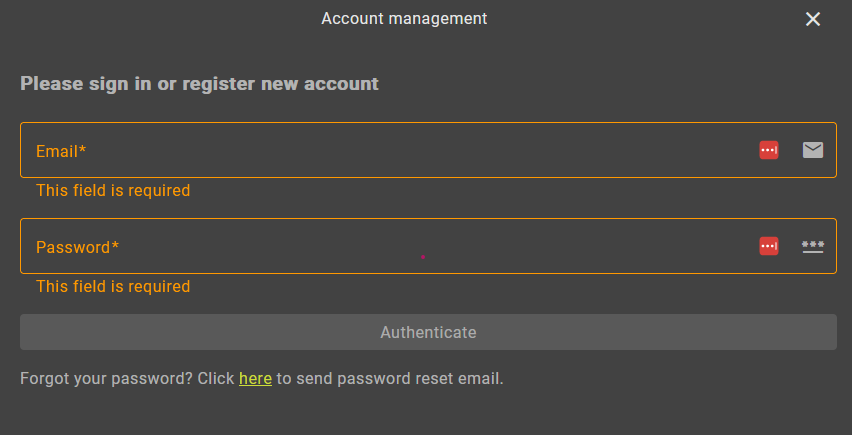
\includegraphics[width=1\textwidth]{attachments/logowanie}
    \caption{Widok panelu logowania}
    \label{fig:logowanie}
\end{figure}

\section{Widok zarządzania wszystkimi POI}
\label{sec:manage}

\begin{figure}[H]
    \centering
    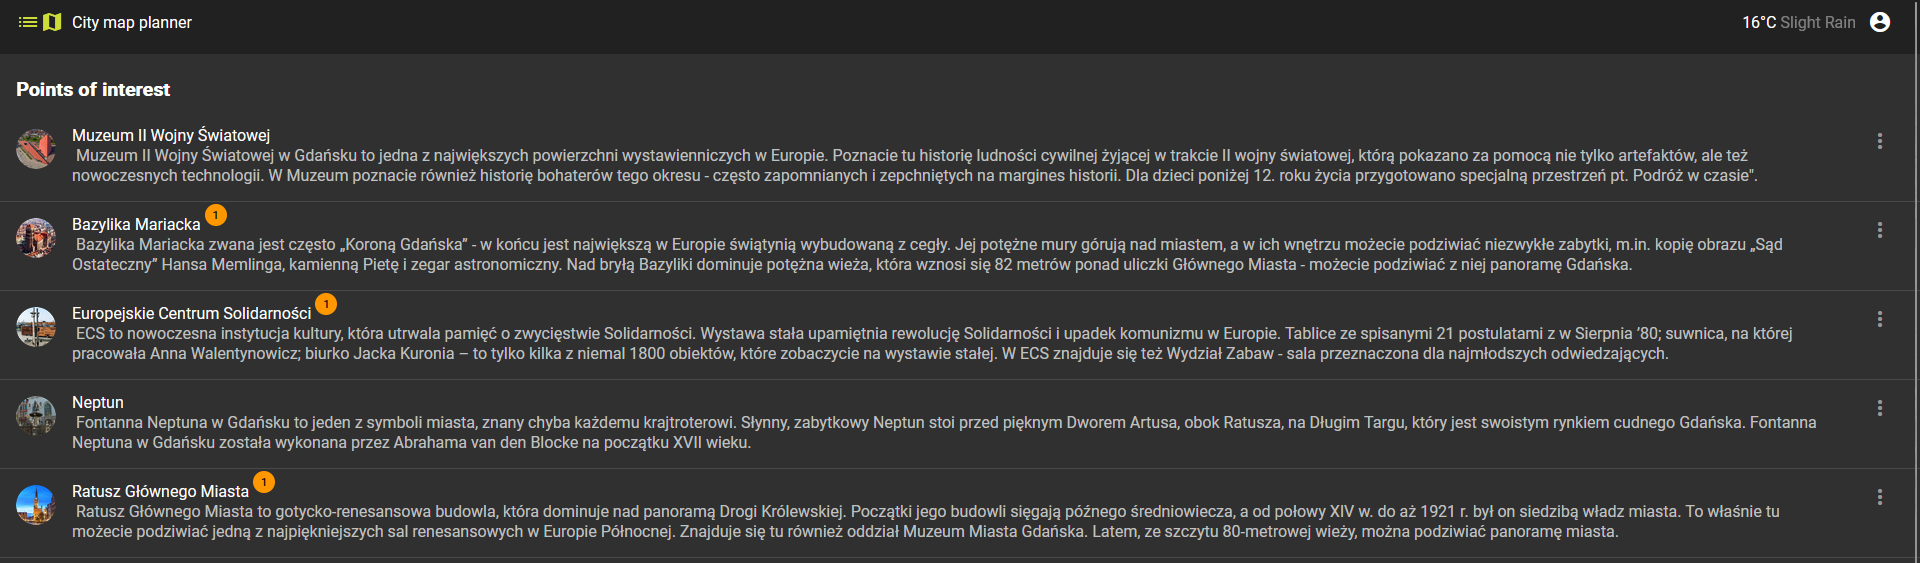
\includegraphics[width=1\textwidth]{attachments/poi-manage}
    \caption{Widok panelu zarządzania wszystkimi POI}
    \label{fig:poi-manage}
\end{figure}

\begin{figure}[H]
    \centering
    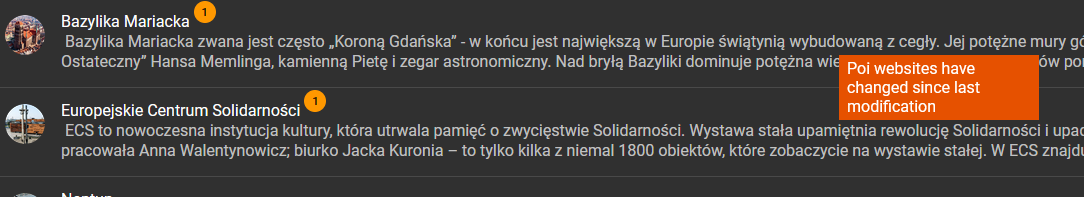
\includegraphics[width=1\textwidth]{attachments/poi-notify}
    \caption{Informacja o potrzebie sprawdzenia aktualności danych}
    \label{fig:ManageNofify}
\end{figure}

\begin{figure}[H]
    \centering
    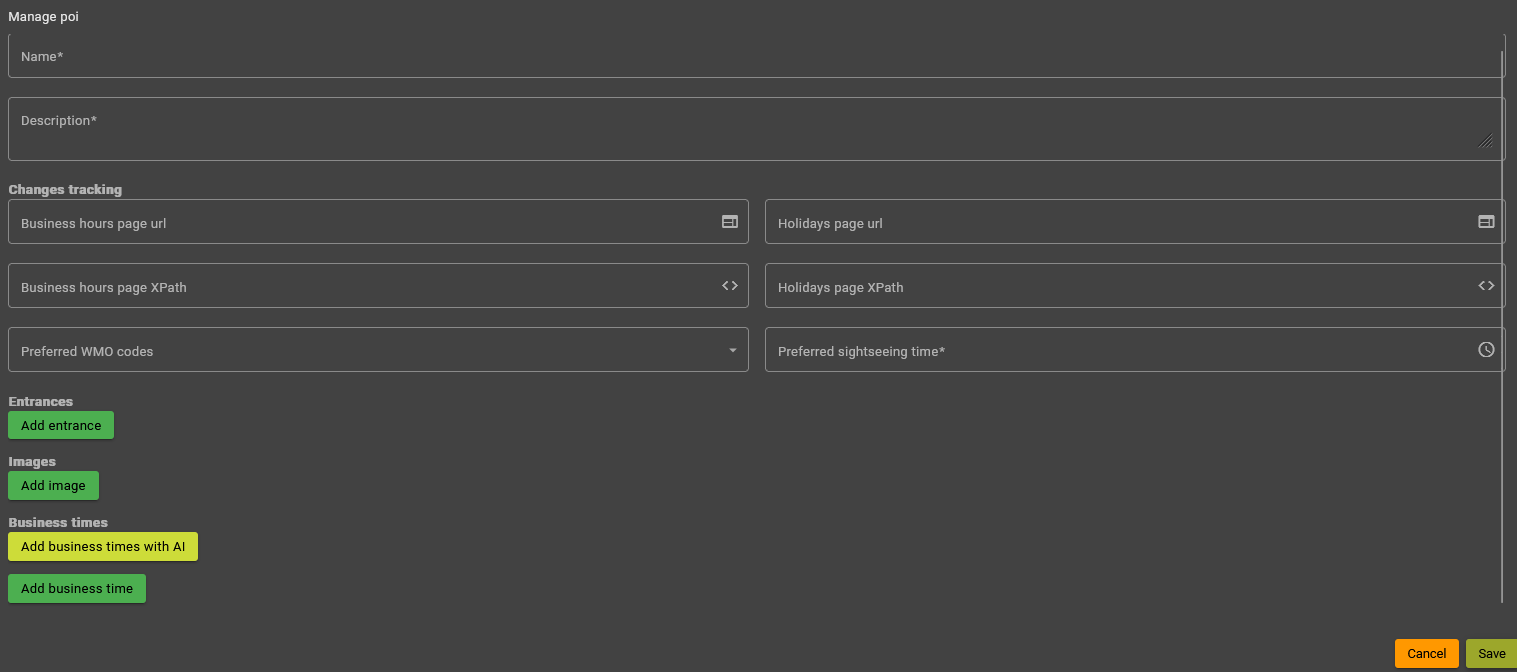
\includegraphics[width=1\textwidth]{attachments/addpoi}
    \caption{Widok panelu dodawania POI}
    \label{fig:ManageNofify}
\end{figure}